This problem is a more general case of the test problem described in
Section \ref{sec:void_to_absorber} in which the transport direction is
not normal to the left boundary; it is a skew direction, for which
$\Omega_i\ge 0,\forall i$, so in 2-D, particles enter through not just the left
boundary, but the bottom boundary as well.
The simulation is again run to $t=1$, but since it is a skew direction,
the wave front is located not along the right boundary but in an ``L''
shape in the strong absorber region.
Table \ref{tab:void_to_absorber_skew} summarizes the test parameters,
where the definition of $s$ is given below.

%-------------------------------------------------------------------------------
\begin{table}[htb]\caption{Skew Void-to-Absorber Test Problem Summary}
\label{tab:void_to_absorber_skew}
\centering
\begin{tabular}{l l}\toprule
\emph{Parameter} & \emph{Value}\\\midrule
Domain & $\mathcal{D} = (0,1)^d$\\
Initial Conditions & $u_0(\x)=0$\\
Boundary Conditions & $u(\x,t)=1,\quad \x\in\partial\mathcal{D}^-,\quad t>0$,\\
   & $\quad\partial\mathcal{D}^-=\{\x\in\partial\mathcal{D}:\mathbf{n}(\x)
       \cdot\mathbf{\Omega}<0\}$\\
Direction & $\mathbf{\Omega} = \left[\frac{1}{\sqrt{2}},\frac{1}{\sqrt{3}},
   \frac{1}{\sqrt{6}}\right]$\\
Cross Section & $\sigma(\x)=\left\{\begin{array}{c l}
   10, & \x\in(\frac{1}{2},1)^d\\
   0,  & \mbox{otherwise}\end{array}\right.$\\
Source & $q(\x,t)=0$\\
Speed & $\speed=1$\\
Exact Solution & $u(\x,t)=\left\{\begin{array}{l l}
   \scalarsolution_{\text{ss}}(\x), & \x-\mathbf{\Omega}t\notin\mathcal{D}\\
   0, & \mbox{otherwise}
   \end{array}\right.$ \\
   & $\scalarsolution_{\text{ss}}(\x) =
       \left\{\begin{array}{l l}
         e^{-10s}, & x\ge\frac{1}{2}, y\ge\frac{1}{2}, z\ge\frac{1}{2}\\
         1,        & \mbox{otherwise}
       \end{array}\right. \eqc$\\
   & with $s$ given by Equation \eqref{eq:s_distance}.\\
\bottomrule\end{tabular}
\end{table}
%-------------------------------------------------------------------------------

The condition $\x-\mathbf{\Omega}t\notin\mathcal{D}$ is equivalent to the
following condition:
\[
   \x-\mathbf{\Omega}t\notin\mathcal{D} \Rightarrow
   \exists i: x_i-\Omega_i t < 0,
\]
where $i$ denotes a coordinate direction index $x$, $y$, or $z$.
The distance traveled in the absorber region, $s$, is computed
by first determining which plane segment of the absorber region
through which the line $\x-\mathbf{\Omega}t$ passes; the coordinate
direction normal to this plane is denoted by $i$ and the other
two by $j$ and $k$. This is determined as follows:
\[
   i: \frac{x_i-\frac{1}{2}}{\Omega_i} = \min\limits_j\left(
      \frac{x_j-\frac{1}{2}}{\Omega_j}\right).
\]
Then, $s$ is computed as follows:
\begin{equation}\label{eq:s_distance}
   s=\sqrt{s_i^2 + s_j^2 + s_k^2}, \quad
   s_i=x_i-\frac{1}{2}, \quad
   s_j=\frac{\Omega_j}{\Omega_i}s_i, \quad
   s_k=\frac{\Omega_k}{\Omega_i}s_i.
\end{equation}

The simulation was run to time $t=1$ with a CFL of $\nu=0.5$ and 16384 cells.
Table \ref{tab:skew_void_to_absorber_run_parameters} summarizes the run parameters
for this test problem.

%-------------------------------------------------------------------------------
\begin{table}[ht]\caption{Skew Void-to-Absorber Test Problem Run Parameters}
\label{tab:skew_void_to_absorber_run_parameters}
\centering
\begin{tabular}{l l}\toprule
\emph{Parameter} & \emph{Value}\\\midrule
Number of Cells & $N_{cell} = 16384$\\
Time Discretization & Explicit Euler, SSPRK33\\
End Time & $t = 1$\\
CFL Number & $\nu = 0.5$\\
Boundary Conditions & Strong Dirichlet with
  $\limiterletter_i^-=\limiterletter_i^+=1$\\\midrule
Entropy Function & $\entropy(\scalarsolution) = \frac{1}{2}\scalarsolution^2$\\
Entropy Residual Coefficient & $\entropyresidualcoef = 0.1$\\
Entropy Jump Coefficient & $\entropyjumpcoef = 0.1$\\\midrule
FCT Solution Bounds & DMP\\
\bottomrule\end{tabular}
\end{table}
%-------------------------------------------------------------------------------

Figures \ref{fig:skew_void_to_absorber_2D_fe} and
\ref{fig:skew_void_to_absorber_2D_ssprk33} show 2-D results for this problem
for explicit Euler and SSPRK33 time discretizations, respectively.

This test problem reveals some multidimensional effects of spurious
oscillations, as one can see in the Galerkin and EV solutions. Comparing
Figures \ref{fig:skew_void_to_absorber_2D_fe} and \ref{fig:void_to_absorber_2D_fe},
one can see that in the skew case, oscillations are now not just perpendicular
to the $x$ axis but also to the $y$ axis, due to the gradients on each
edge of the absorber region. One can also see some faint oscillations
propagating from the corner of the absorber region. It is also interesting
to note a circular effect centered at the lower left corner of the domain;
this is presumed to be due to interactions between the horizontal and
vertical oscillations. Also note that in this problem, the wave front
is not at the right edge of the domain as it was in non-skew test
problem; instead, the wave front is in the absorber region, which
one can clearly see in the exact solution. The wave front is an ``L''
shape since with the skew, particles/photons now also enter the domain
from the lower boundary of the domain. The conclusion of the results
is the same as before: FCT eliminates the spurious oscillations apparent
in the Galerkin and EV solutions and is sharper than the low-order
solution. The advantage of using FCT over the low-order scheme is
less evident in these results simply because the wave front is
in the absorber region, where the solution is already very small;
thus the gradient is more difficult to see.

Figure \ref{fig:skew_void_to_absorber_visc} shows the low-order
and entropy viscosity profiles for SSPRK33. As in the normally-incident
void-to-absorber test problem, the highest entropy viscosity occurs
at the corner of the absorber region, and is otherwise large on
the boundaries of the absorber region.

%-------------------------------------------------------------------------------
\begin{figure}[ht]
   \centering
   \begin{subfigure}{0.3\textwidth}
      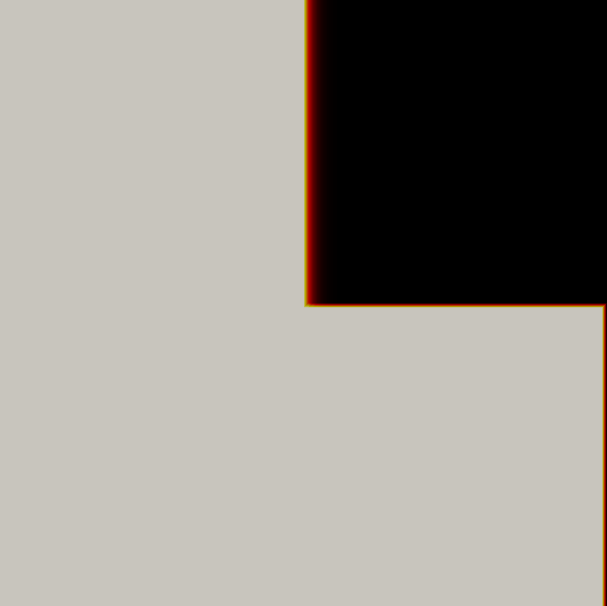
\includegraphics[width=\textwidth]
        {\contentdir/results/transport/skew_void_to_absorber/images/Exact.png}
      \caption{Exact}
   \end{subfigure}
   \begin{subfigure}{0.3\textwidth}
      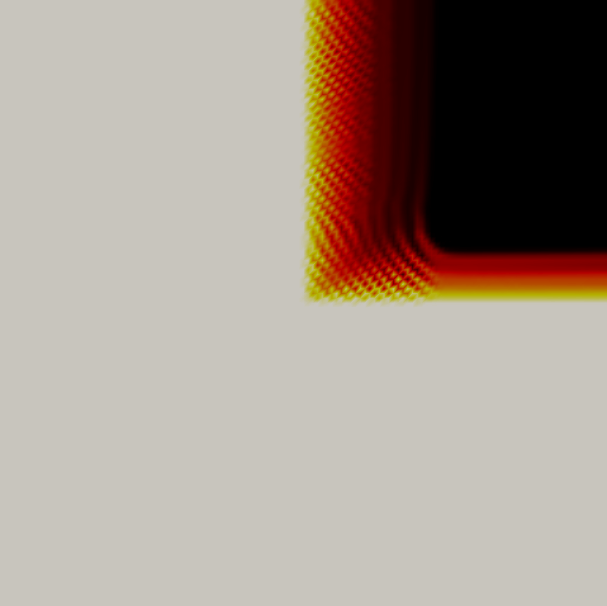
\includegraphics[width=\textwidth]
        {\contentdir/results/transport/skew_void_to_absorber/images/GalFCT_FE.png}
      \caption{Galerkin FCT}
   \end{subfigure}
   \begin{subfigure}{0.3\textwidth}
      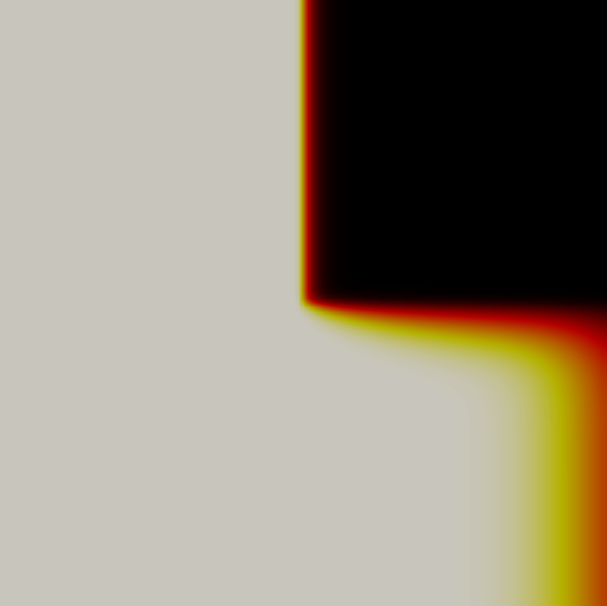
\includegraphics[width=\textwidth]
        {\contentdir/results/transport/skew_void_to_absorber/images/Low_FE.png}
      \caption{Low-order}
   \end{subfigure}
   \begin{subfigure}{0.3\textwidth}
      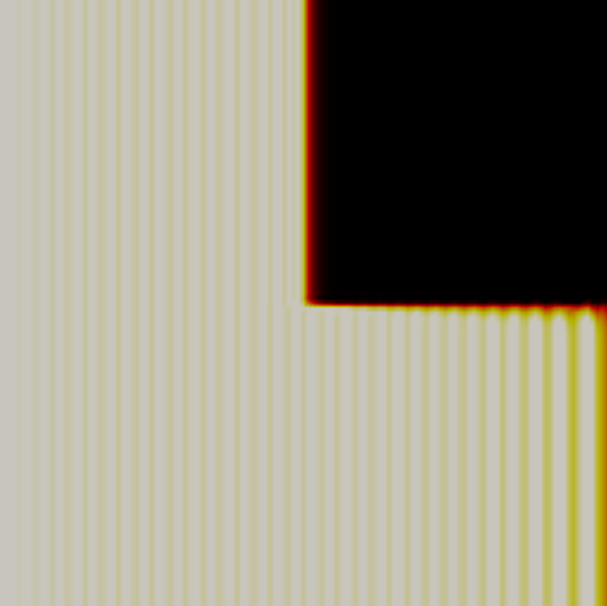
\includegraphics[width=\textwidth]
        {\contentdir/results/transport/skew_void_to_absorber/images/EV_FE.png}
      \caption{Entropy Viscosity}
   \end{subfigure}
   \begin{subfigure}{0.3\textwidth}
      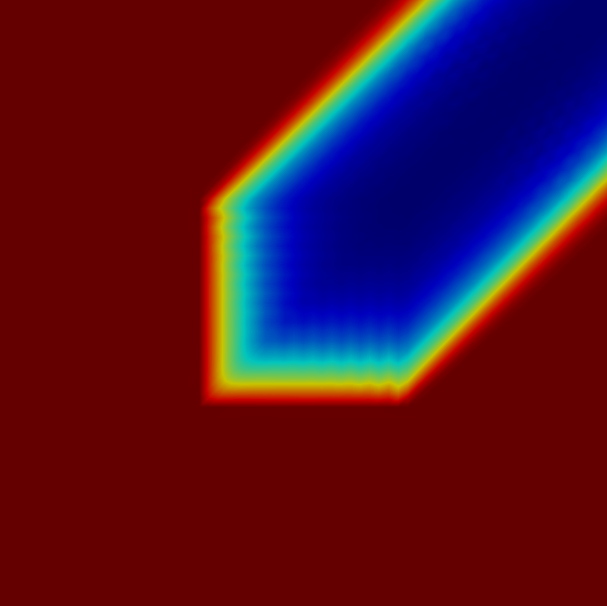
\includegraphics[width=\textwidth]
        {\contentdir/results/transport/skew_void_to_absorber/images/EVFCT_FE.png}
      \caption{Entropy Viscosity FCT}
   \end{subfigure}
   \caption{Comparison of Solutions for the Skew Void-to-Absorber Test Problem
     Using Explicit Euler Time Discretization and DMP Solution Bounds with 16384 Cells}
   \label{fig:skew_void_to_absorber_2D_fe}
\end{figure}
%-------------------------------------------------------------------------------
%-------------------------------------------------------------------------------
\begin{figure}[ht]
   \centering
   \begin{subfigure}{0.3\textwidth}
      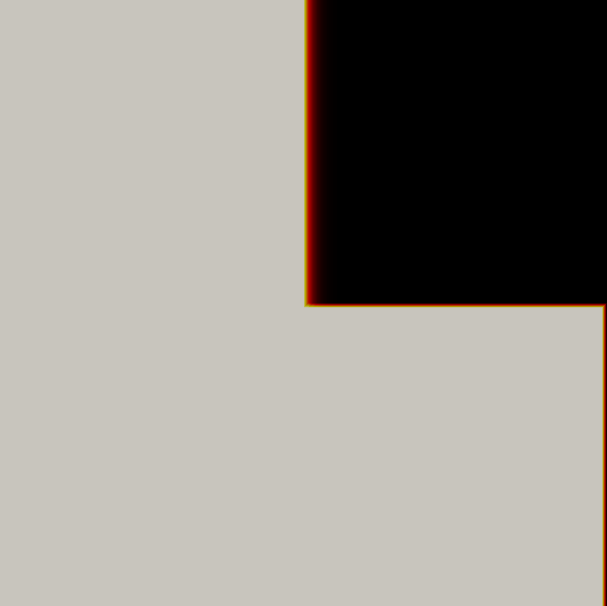
\includegraphics[width=\textwidth]
        {\contentdir/results/transport/skew_void_to_absorber/images/Exact.png}
      \caption{Exact}
   \end{subfigure}
   \begin{subfigure}{0.3\textwidth}
      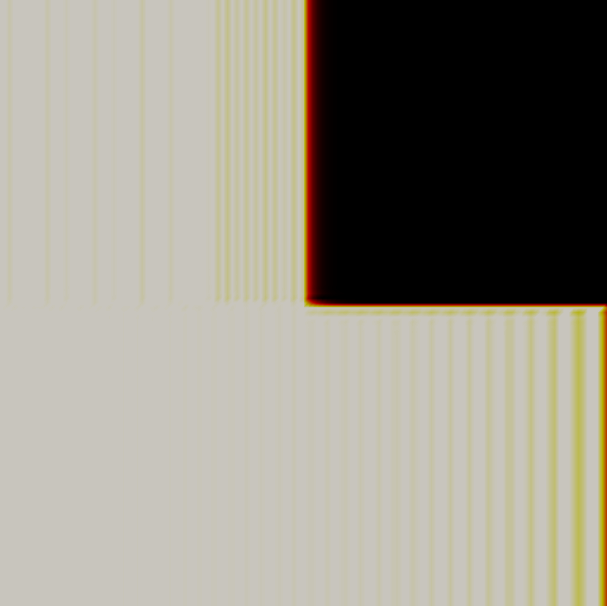
\includegraphics[width=\textwidth]
        {\contentdir/results/transport/skew_void_to_absorber/images/Gal_SSPRK33.png}
      \caption{Galerkin}
   \end{subfigure}
   \begin{subfigure}{0.3\textwidth}
      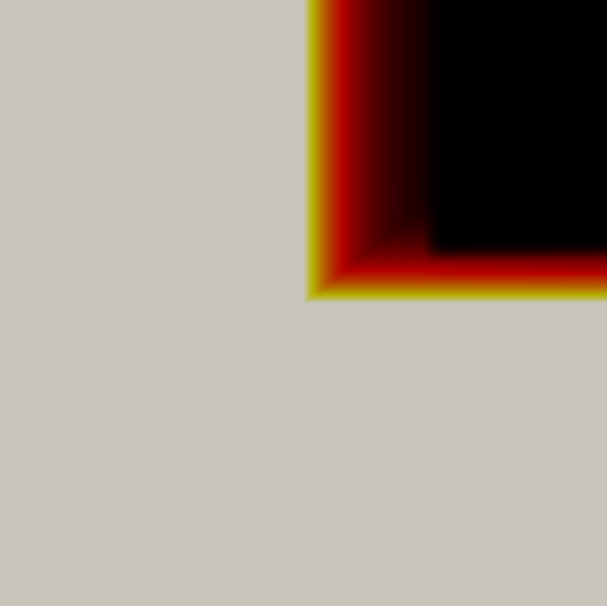
\includegraphics[width=\textwidth]
        {\contentdir/results/transport/skew_void_to_absorber/images/GalFCT_SSPRK33.png}
      \caption{Galerkin FCT}
   \end{subfigure}
   \begin{subfigure}{0.3\textwidth}
      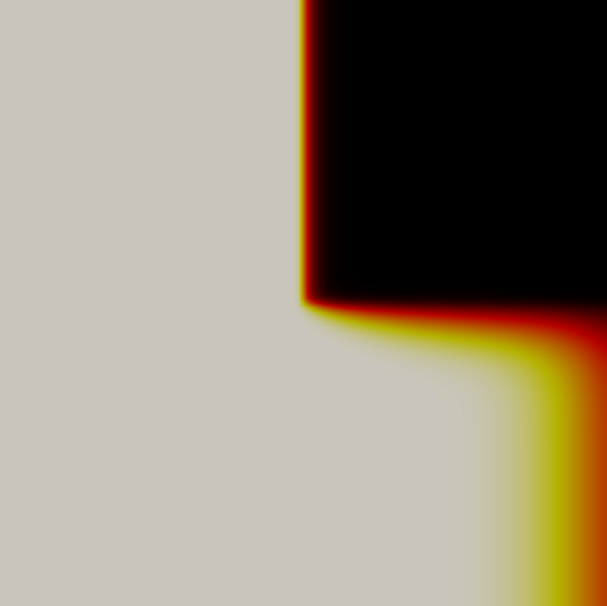
\includegraphics[width=\textwidth]
        {\contentdir/results/transport/skew_void_to_absorber/images/Low_SSPRK33.png}
      \caption{Low-order}
   \end{subfigure}
   \begin{subfigure}{0.3\textwidth}
      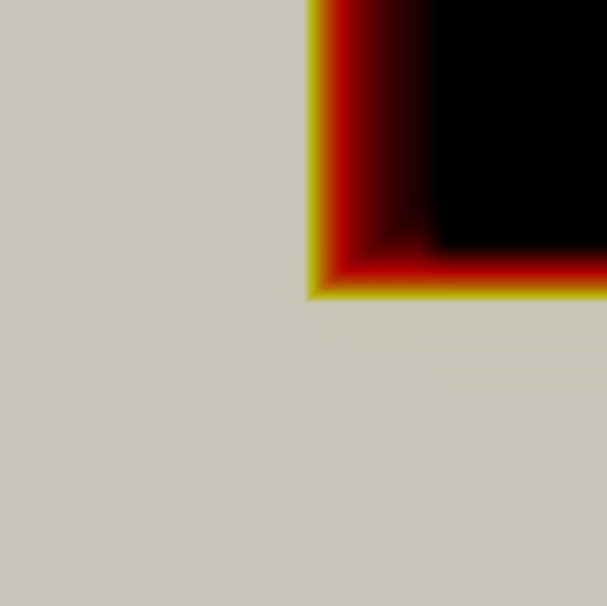
\includegraphics[width=\textwidth]
        {\contentdir/results/transport/skew_void_to_absorber/images/EV_SSPRK33.png}
      \caption{Entropy Viscosity}
   \end{subfigure}
   \begin{subfigure}{0.3\textwidth}
      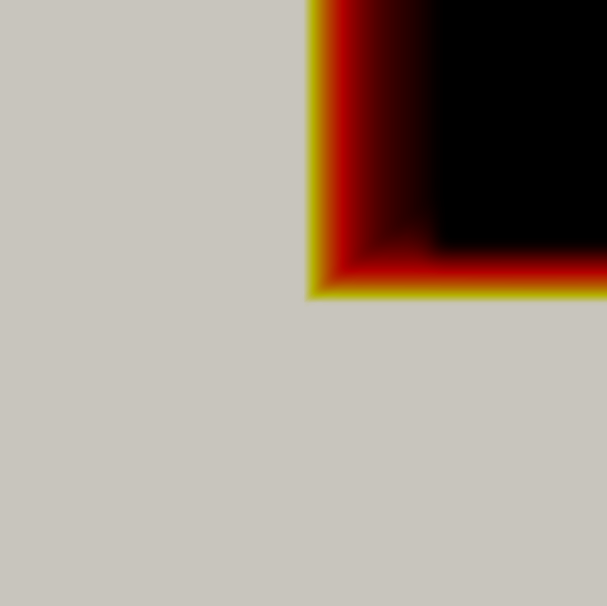
\includegraphics[width=\textwidth]
        {\contentdir/results/transport/skew_void_to_absorber/images/EVFCT_SSPRK33.png}
      \caption{Entropy Viscosity FCT}
   \end{subfigure}
   \caption{Comparison of Solutions for the Skew Void-to-Absorber Test Problem
     Using SSPRK33 Time Discretization and DMP Solution Bounds with 16384 Cells}
   \label{fig:skew_void_to_absorber_2D_ssprk33}
\end{figure}
%-------------------------------------------------------------------------------
%-------------------------------------------------------------------------------
\begin{figure}[ht]
   \centering
   \begin{subfigure}{0.45\textwidth}
      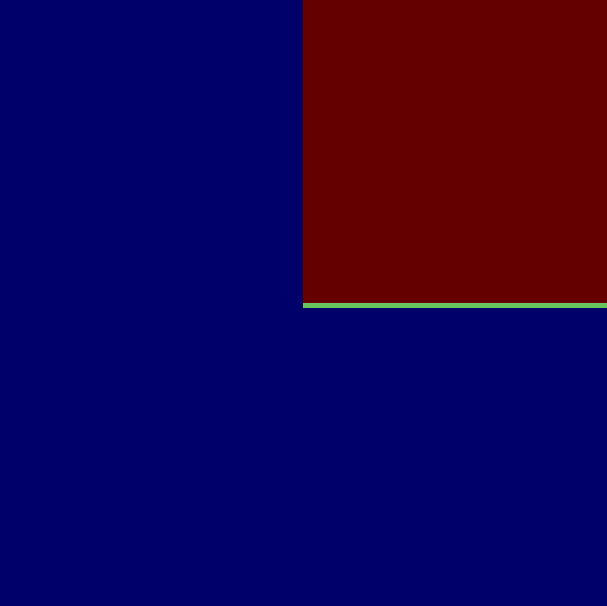
\includegraphics[width=\textwidth]
        {\contentdir/results/transport/skew_void_to_absorber/images/low_viscosity_SSP3_linearscale.png}
      \caption{Low-order viscosity}
   \end{subfigure}
   \begin{subfigure}{0.45\textwidth}
      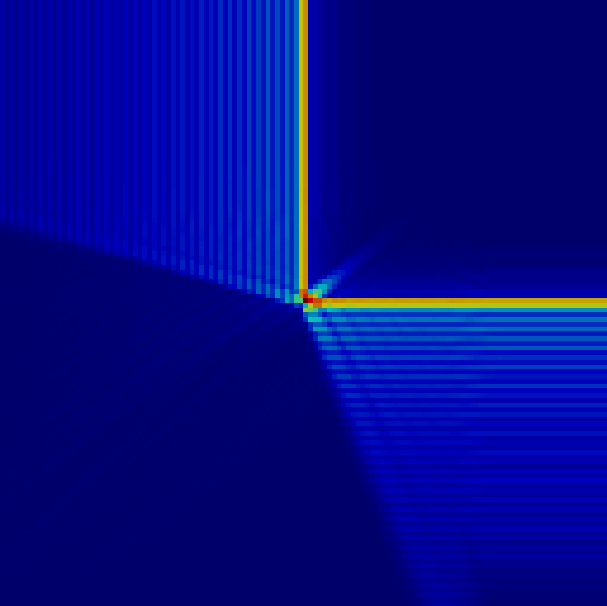
\includegraphics[width=\textwidth]
        {\contentdir/results/transport/skew_void_to_absorber/images/entropy_viscosity_SSP3_linearscale.png}
      \caption{Entropy viscosity}
   \end{subfigure}
   \caption{Viscosity Profiles for the the Skew Void-to-Absorber Test Problem
     Using SSPRK33 Time Discretization}
   \label{fig:skew_void_to_absorber_visc}
\end{figure}
%-------------------------------------------------------------------------------

\clearpage
